\section{Intégration dans NewMadeleine}

Pour cette partie, j'ai utilisé ce que j'ai appris en cours :

5 Intégration dans NewMadeleine
5.1 Présentation des détails de NewMadeleine

\begin{itemize}
  \item De \emph{Programmation des Architectures Parallèles} (PAP) et de \emph{Langages du Parallélisme} pour la compréhension du fonctionnement interne des bibliothèques \emph{MPI} et pour aborder différentes problématiques liées à la programmation parallèle.
  \item De \emph{Projet de Programmation} (PdP) et de \emph{Lecture d'article et documentation scientifique} pour effectuer les recherches bibliographiques.
  \item D'\emph{Analyse des données} pour traiter les courbes.
  \item D'\emph{algo des structure de données} pour m'aider à comprendre les file \emph{lock-free} et \emph{wait-free}.
  % \item Les cours de \emph{CISD} m'ont été utiles pour HPC en général.
\end{itemize}

\subsection{Présentation détaillée de NewMadeleine}

La bibliothèque de communications \emph{NewMadeleine} propose plusieurs interfaces disponibles pour l'utilisateur.
Parmi les interfaces les plus importantes, on trouve \emph{sendrecv} pour envoyer et recevoir des données,
\emph{coll} pour les opérations collectives,
\emph{MPI} qui implémente le standard \emph{MPI} en utilisant les interfaces \emph{sendrecv} et \emph{coll},
et \emph{rpc} qui permet le support des \emph{RPC}.


Pour ce stage, nous avons principalement utilisé l'interface \emph{sendrecv}.

Cette interface permet à l'utilisateur de manipuler des requêtes de communication
en soumettant des tâches au coeur de la bibliothèque \emph{nm_core}.

Ces tâches, nommé \emph{core_task}, peuvent être de différents types, tels que la soumission d'une requête,
la complétion des paquets, l'exécution de handlers, etc.
Les tâches du coeur fonctionnent dans des sections critiques en utilisant un verrou nommé \emph{core_lock}.

La bibliothèque s'occupe automatiquement de la génération des requêtes et des paquets,
du découpage des données en tronçons et de l'application des stratégies d'optimisation.

Le coeur de la bibliothèque s'occupe de l'exécution des tâches et de la progression des communications grâce à la fonction \emph{nm_schedule}.
Cette fonction peut être déclenchée à partir d'une interface (e.g. la fonction \emph{MPI_Test}).

Pour effectuer les communications, il est possible d'utiliser différents réseaux ou autres technologies qui utilisent une même interface, appelés \emph{drivers}. % historiquement appelé minidriver
Au cours de ce stage, nous nous sommes concentrés sur les parties qui s'occupent de la progression des communications et des drivers.
Nous ne rentrerons donc pas dans les détails concernant les différentes interfaces, les stratégies, \emph{Pioman}, etc.

Dans les parties que nous avons manipulées lors du stage, les paquets sont représentés par des "paquet wrappers",
que nous abrégerons par "\emph{pw}" par la suite.
Les \emph{pw} possèdent toutes les informations nécessaires pour l'envoi ou la réception de tronçons de données et
pour que la tâche de complétion de la requête puisse remonter les données à l'utilisateur.

La progression se fait donc grâce à la fonction \emph{nm_schedule}, qui effectue les étapes suivantes :

\begin{enumerate}
  \item Commence par exécuter les tâches en utilisant le verrou \emph{core_lock},
  \item Puis elle fait progresser les \emph{pw} de réception,
  \item Puis elle fait progresser les \emph{pw} d'envois,
  \item Elle déclenche le prefetch si nécessaire (nous ne rentrerons pas dans le détail pour le prefetch),
  \item Puis elle exécute de nouveau les tâches dans le cas où de nouvelles tâches ont été soumises par la progression des \emph{pw},
  \item Enfin, elle envoie, si nécessaire, des événements aux interfaces supérieures.
\end{enumerate}

Tous les drivers suivent une interface qui permet :

\begin{itemize}
  \item D'instancier le driver grâce à une fonction \emph{init} qui donne une URL qui faut partagée avec les autres processus pour initier une connexion. % puk_context_t context
  \item D'instancier une connexion grâce à une fonction \emph{connect} qui prend en paramètre l'URL d'un autre processus avec lequel on souhaite communiquer.
  La connexion est bien sûr essentielle pour communiquer et une instance d'un driver peut avoir plusieurs connexions simultanées.
  \item De poster une réception ou un envoi pour les trois types de représentation de données (iovec, buffer, data).
  Seul un des types peut être implémenté dans le driver final.
  Les fonctions sont \emph{send_XX_post} et \emph{recv_XX_post}, où "XX" est remplacé par les trois types \emph{iov}, \emph{buf} et \emph{data}.
  Nous utiliserons les termes "poster une réception" et "poster un envoi" par la suite.
  \item De scruter une réception ou un envoi avec \emph{send_poll}, \emph{recv_poll_one} et \emph{recv_buf_poll}.
  Nous utiliserons les termes "scruter une réception" et "scruter un envoi" par la suite.
  \item De scruter une réception de n'importe quelle source avec \emph{recv_probe_any}.
  \item De libérer une connexion et le driver en entier avec toutes les connexions respectivement avec les fonctions \emph{disconnect} et \emph{close}.
  \item De réaliser diverses actions, comme \emph{send_buf_get} pour récupérer l'adresse d'un nouveau buffer,
  \emph{recv_buf_release} pour le libérer, \emph{get_rdv_data} et \emph{set_rdv_data} pour les rendez-vous, etc.
\end{itemize}

Les trois types différents représentent des données de manière distincte :
\begin{itemize}
  \item Le type "data" représente une zone mémoire contiguë allouée par l'utilisateur.
  \item Le type "buffer" représente également une zone mémoire contiguë, mais elle est allouée par le driver.
  \item Le type "iovec" représente un vecteur de plusieurs zones mémoire qui peuvent être de tailles différentes,
  donc non continues.
\end{itemize}

Les paquets sont distingués en deux catégories :
les petits qui rentrent entièrement dans l'espace mémoire utilisé pour la communication,
et les gros qui ne rentrent pas entièrement et sont donc coupés en tronçons pour être envoyés un par un.
% req.data split in req_chunk
Les drivers ont une implémentation différente pour les petits et les gros paquets, donc deux instances sont manipulées.

Pour manipuler les drivers, la bibliothèque utilise une représentation nommée \emph{nm_drv} que nous abrégeons \emph{drv}.
Ce \emph{drv} est donc instancié et va s'occuper d'instancier un driver pour les petits paquets et un pour les gros paquets.
Il va les paramétrer et les stocker avec leur URL dans son instance.
Par la suite, nous allons modifier sa structure pour qu'il puisse stocker des listes en plus.
Un \emph{drv} permet donc de faire la jonction entre les drivers et le coeur de la bibliothèque.
La bibliothèque peut accéder au URL pour les partager avec d'autres processus.

Le core possède deux listes de \emph{pw} pour la réception et pour l'envoi,
qui sont \emph{pending_send_list} et \emph{pending_recv_list}.

Ces listes possèdent :
\begin{itemize}
  \item Un \emph{pw} pour chaque connexion de chaque instance de driver.
  \item Un \emph{pw} supplémentaire pour la liste de réception pour chaque instance de driver qui supporte les petits
  paquets et qui implémente la fonction \emph{recv_probe_any}.
  En effet, seuls les petits paquets peuvent avoir cette fonction.
  Le \emph{pw} supplémentaire est donc posté dans le cas où l'on n'a pas posté de réception, mais qu'on en reçoit une.
\end{itemize}

Le \emph{pw} connaît l'instance du driver à laquelle il est rattaché.
Dans la fonction \emph{nm_schedule}, faire progresser les \emph{pw} de réception consiste à parcourir chaque \emph{pw} de la liste
de réception pour scruter une réception ou pour poster une réception dans le cas du \emph{pw} dédié à la réception des paquets non posté.
Si la scrutation est positive, une tâche du coeur (\emph{core_task}) de complétion sera soumise.
Lorsque le \emph{nm_schedule} fait progresser les \emph{pw} d'envoi, le fonctionnement est similaire à la réception,
mais sans la gestion des paquets non posté qui n'existe que pour la reception des petit paquets.

Le polling se fait donc par des appels réguliers à \emph{nm_schedule} depuis \emph{Pioman}, ou par des appels à \emph{MPI_Test} ou \emph{MPI_Wait}.

J'ai eu des difficultés de compréhension pour le cycle de vie des \emph{pw} qui est un peu complexe car
ils passent à plusieurs endroits (les listes, les core tasks, ils sont réutilisés quand la tâche est traitée...).

\subsection{Modifications}

\subsubsection{Ajout de drivers}

Lors de ce stage, nous nous concentrons donc sur le driver qui effectue les communications en mémoire partagée,
que nous appellerons \emph{driver shm}.

Nous avons donc ajouté deux drivers basés sur le driver \emph{shm}.
Le premier est le driver \emph{sig_shm}, qui utilise les signaux comme abstraction des uintr.
Ce driver \emph{sig_shm} a été très utile lorsque nous n'avions pas accès à la machine qui supporte les \uintr{},
ainsi que pour faciliter le débogage.
Le second est le driver \emph{uintr_shm}, qui utilise les \uintr{}.

Ces deux drivers initialisent leur handler lors de l'initialisation (\emph{init}) et libèrent la mémoire à la terminaison (\emph{close}).
Chaque driver utilise son propre handler, soit de signal, soit d'interruption, qui permet de vérifier s'il existe un \emph{handler de driver} défini,
et le cas échéant, de l'appeler.

Un \emph{handler de driver} est un nouveau type de handler qui est défini par une fonction \emph{set_handler},
que nous avons ajoutée à l'interface des drivers.
Cette fonction est appelée lors de l'instanciation du \emph{drv},
juste après avoir instancié le driver, et uniquement si le driver supporte les \emph{handler de driver}.

Le \emph{handler de driver} est fourni par le \emph{drv} lui-même et défini dans le \emph{drv}.
Il permet de gérer la progression des tâches, comme nous le verrons dans la section \ref{progression}.

Ces deux drivers ont deux variantes, une pour les petits paquets et une pour les gros paquets.

Pour les signaux, on utilise \emph{SIGUSR1} pour les petits paquets et \emph{SIGUSR2} pour les gros paquets,
avec un handler de signal distinct pour chacun.

Pour les \uintr{}, on utilise le vecteur 6 pour les petits paquets et le vecteur 8 pour les gros paquets.
Comme nous ne pouvons définir qu'un seul handler pour les deux vecteurs,
nous avons ajouté un mécanisme qui permet d'appeler un handler local au driver à partir d'un handler global.
Ainsi, chaque driver possède son propre handler, que ce soit de signal ou d'interruption, capable d'appeler le \emph{handler de driver}.

Pour ajouter le driver avec les \uintr{},
nous avons ajouté l'argument \emph{--enable-uintr} dans le fichier \emph{configure.ac} de \emph{NewMadeleine}.
Le fichier \emph{configure.ac} est utilisé par \emph{Autotools} pour la génération d'un \emph{Makefile}.
L'argument permet d'activer le support des \uintr{} uniquement lorsque le compilateur et la machine les supportent.
De plus, nous avons modifié le fichier \emph{Makefile.in} en ajoutant les bons flags de compilation nécessaires pour le support des \uintr{}.

L'envoi des signaux ou des interruptions se fait au moment de scruter une réception ou un envoi.
L'objectif final est que l'émetteur envoie une interruption au récepteur pour l'avertir qu'il peut faire une scrutation.
Le récepteur fait sa scrutation et envoie une interruption à l'émetteur pour le prévenir qu'il peut recevoir la suite.

Dans le cas des petits paquets, l'émetteur ne renvoie pas d'interruption car la communication est terminée.
En revanche, dans le cas des gros paquets, les allers-retours continuent jusqu'à la fin de la communication.
Ainsi, on ne réalise des scrutations que lorsque cela est nécessaire.

Actuellement, nous envoyons une interruption ou un signal seulement au moment de scruter l'envoi car le support des gros paquets ne fonctionne pas encore.

On effectue l'envoi de l'interruption au moment de la scrutation car la bibliothèque fait toujours une scrutation après avoir posté une communication.

\subsubsection{Progression à partir des handlers}
\label{progression}

Pour faire progresser les communications à partir des handlers et non par des scrutations répétées,
nous commençons par ne plus ajouter les \emph{pw} qui sont liés à un driver possédant un \emph{handler} dans les listes \emph{pending_send_list} et \emph{pending_recv_list}.

Nous avons donc ajouté deux nouvelles listes de \emph{pw} pour la réception et pour l'envoi dans le \emph{drv}.
Ces listes seront utilisées spécifiquement par le \emph{handler de driver}.

Le \emph{handler de driver} est défini dans le \emph{drv} et est nommé \emph{drv_handler}.
Il est déclenché par le handler local des drivers lorsqu'un signal ou une interruption est reçu.

Lors du déclenchement, celui-ci connaît l'instance du \emph{drv} et effectue une progression.
Il commence par tenter de faire progresser les tâches du coeur si le verrou est \emph{core_lock}.
Pour ce faire, il essaie de prendre le verrou \emph{core_lock} avec la fonction \emph{try_lock}.
Si le verrou est pris, alors les tâches du coeur sont exécutés. Sinon, on passe à l'étape suivante.

Il est important de rappeler qu'on ne peut pas attendre dans un handler de signal ou d'interruption,
et c'est précisément ce genre de handler qui déclenche le \emph{handler de driver}.
Donc, plutôt que d'attendre, le \emph{handler de driver}.

Ensuite, nous essayons de faire progresser tous les éléments des nouvelles liste de \emph{pw}.
Pour cela, nous appelons les mêmes fonctions que celles utilisées dans le \emph{nm_schedule} principal.
Ces fonctions ont été modifiées pour utiliser la liste appropriée en fonction de si le \emph{pw} prend en charge les handlers ou non.
Avant de passer à la progression de l'élément suivant, nous essayons de faire progresser les tâches du coeur si possible.
Si ce n'est pas possible, nous ajoutons l'instance du \emph{drv} dans une nouvelle file de \emph{drv} en attente (\emph{pending_drv}) qui se trouve dans le \emph{nm_core}.

Une fois que nous avons fait progresser tous les éléments une fois, nous pouvons déterminer s'il faut le faire une nouvelle fois.
Pour cela, il faut que les tâches du coeur aient pu progresser pour que les \emph{pw} soient disponibles et qu'il soit nécessaire de faire une seconde progression.
Il est important de noter que nous sommes limités en nombre de \emph{pw} car nous ne pouvons pas effectuer d'allocation dans un handler de signal ou d'interruption.
Une allocation, par exemple avec \emph{malloc}, n'est pas "async safe" et peut entraîner une attente,
ce qui n'est pas autorisé dans un handler.

Une seconde progression est nécessaire dans le cas où plusieurs interruptions ont été reçues en même temps.
Étant donné que nous ne pouvons pas savoir combien d'interruptions ont été reçues car elles s'écrasent,
nous utilisons la fonction \emph{recv_probe_any} du driver pour déterminer s'il faut refaire une progression.
Cependant, l'utilisation de \emph{recv_probe_any} fonctionne uniquement pour les drivers des petits paquets.
Pour les drivers des gros paquets, nous ne faisons qu'une seule progression pour le moment.
Le support des gros paquets n'est pas encore terminé et présente encore des bugs.

Nous avons donc vu que nous utilisons une file de \emph{drv} en attente,
car une partie de la progression se fait dans une zone critique qui nécessite la prise d'un verrou.
Comme nous ne pouvons pas attendre dans un handler, nous ne pouvons pas garantir la prise du verrou,
donc nous remettons le traitement à plus tard grâce à cette file.

Les \emph{drv} de cette file sont traités au moment où un thread relâche le verrou du core ou lorsque nous recevons de nouveau une interruption.
Le fait de traiter les progressions des \emph{drv} peut entraîner des conflits si le handler est déclenché et
fait également une progression, donc il faut protéger cette progression.
Pour ce faire, nous avons utilisé l'opération atomique \emph{compare and swap} pour nous assurer d'être seuls à faire la progression.
Si le handler échoue le \emph{compare and swap}, alors il ajoute l'instance du \emph{drv} à la file de \emph{drv} en attente.

\subsubsection{File de \emph{drv} en attente}

La file de \emph{drv} en attente est une file dont les opérations d'enfiler et de défiler (enqueue et dequeue) sont effectuées sans verrou (\emph{lock-free}).
Ces files \emph{lock-free} sont donc très utilisées dans \emph{NewMadeleine}.
Le principe de fonctionnement consiste à déterminer si quelqu'un d'autre modifie la file en même temps, et si c'est le cas, on attend.
Cependant, cela peut entraîner une problématique d'état bloquant (deadlock en anglais),
que nous avons rencontrée lors de nos tests.

L'état bloquant survient car le thread qui est en train de modifier la file est interrompu,
et le handler veut également modifier la file, donc il attend que le thread interrompu ait fini, ce qui n'arrive jamais.
Pour résoudre ce problème, nous avons besoin d'une file sans attente (\emph{wait-free}).

\subsubsection{File \emph{lock-free} et \emph{wait-free}}

J'ai donc effectué une recherche bibliographique pour trouver une implémentation dans la littérature.

L'origine des files \emph{wait-free} provient des files \emph{lock-free}.
La première file \emph{lock-free} est celle de Michael \& Scott \cite{MICHAEL19981}, qui est nommée \emph{MSQueue} dans la littérature.

Une première file \emph{wait-free}, basée sur le même fonctionnement que la \emph{MSQueue},
est proposée par A. Kogan \& E. Petrank \cite{10.1145/1941553.1941585} et est nommée \emph{KPQueue}.
Cependant, cette file présente des performances très limitées et ne passe pas à l'échelle.
Plusieurs autres files ont été proposées pour améliorer les performances,
comme la \emph{FCQueue} de D. Hendler \& I. Incze \& N. Shavit \& M. Tzafrir \cite{10.1145/1810479.1810540}.
Cette file est \emph{wait-free} grâce à l'utilisation de verrous et offre des performances raisonnables.
Cependant, elle est basée sur des listes chaînées, ce qui signifie que les éléments sont alloués lors de l'insertion.
Étant donné que nous ne pouvons pas utiliser d'allocateur dans un handler d'interruption,
cette file ne convient pas à notre cas d'utilisation.

Les files \emph{CCQueue} et \emph{H-Queue} sont basées sur la même idée que la file \emph{FCQueue}, mais elles peuvent passer à l'échelle.
Elles ont été proposées par P. Fatourou \& N. D. Kallimanis \cite{10.1145/2370036.2145849} et elles rencontrent les mêmes problèmes que la \emph{FCQueue}.

La file \emph{SimQueue} (également appelée \emph{FKQueue}) est une file \emph{lock-free} et \emph{wait-free} basée sur des listes chaînées,
donc ne nous convient pas à notre cas et est moins performante que la \emph{FCQueue}.
Elle présente aussi des problèmes de libération de mémoire, comme décrit par P. Ramalhete \& A. Correia \cite{10.1145/3155284.3019022}.
Cette file a été proposée par P. Fatourou \& N. D. Kallimanis \cite{10.1145/1989493.1989549}.

Les mêmes auteurs ont également proposé \emph{PSim} \cite{Fatourou2014}, qui est basé sur \emph{SimQueue} mais avec des améliorations pour une meilleure efficacité.
Cependant, il semblerait qu'il présente toujours les problèmes de libération de mémoire décrits par P. Ramalhete \& A. Correia.
L'accès à l'article est payant, mais selon des articles plus récents, \emph{PSim} montre des performances relativement bonnes.

Une autre file \emph{wait-free} qui présente de très bonnes performances est la \emph{WFQueue} (aussi connue sous le nom de \emph{YMC queue}),
proposée par C. Yang \& J. Mellor-Crummey \cite{10.1145/3016078.2851168}.
Elle est basée sur des listes chaînées mais pourrait également rencontrer les problèmes de libération de mémoire décrits par P. Ramalhete \& A. Correia.

P. Ramalhete \& A. Correia présentent une file nommée \emph{CRTurn} \cite{10.1145/3155284.3019022}, qui est \emph{wait-free} et cherche à résoudre les problèmes de libération de mémoire.
Leur implémentation n'est pas très performante, mais ils discutent d'une grande partie des files précédentes et les regroupent dans un même dépôt \emph{Github}, avec un moyen de mesurer leurs performances.

En 2019, R. Nikolaev propose une file \emph{lock-free} uniquement, nommée \emph{SCQ} \cite{10.4230/lipics.disc.2019.28}.
Elle est inspirée de la file \emph{CRQ}, mais elle est plus efficace en termes de mémoire et évite les problèmes de \emph{livelocks}.
La file \emph{CRQ} est une file \emph{lock-free} performante qui utilise l'opération atomique \emph{compare and swap} sur 2 mots contigus en mémoire (\emph{CAS2}),
qui n'est pas disponible sur tous les CPU.
\emph{CRQ} est proposée par A. Morrison \& Y. Afek \cite{10.1145/2517327.2442527}.
\emph{SCQ} n'utilise pas les \emph{CAS2} et parvient à des performances similaires à \emph{CRQ}.
De plus, \emph{SCQ} passe très bien à l'échelle.

En 2022, la file \emph{wCQ} est proposée par R. Nikolaev \& B. Ravindran \cite{10.1145/3490148.3538572}.
Basée sur \emph{SCQ}, elle est en plus \emph{wait-free}.
Cette file présente de bonnes performances et passe très bien à l'échelle.
Les auteurs se sont appuyés sur le dépôt \emph{GitHub} de P. Ramalhete \& A. Correia pour y ajouter leur implémentation dans ce nouveau dépôt \cite{wCQ}.

Pendant mes recherches, mon tuteur de stage, \emph{Alexandre Denis},
a amélioré son implémentation de la \emph{lfqueue} pour "Lock-Free Queue".
Dans cette file, les éléments qui peuvent y être insérés sont des pointeurs.
Il a utilisé une technique très astucieuse consistant à utiliser les 16 premiers bits non utilisés des pointeurs
pour compter le nombre de modifications qu'a subi une entrée de la file.
Ainsi, s'il y a eu un changement entre la lecture et l'écriture atomique,
il sait qu'une autre opération modifie la liste et peut réagir en conséquence.
Cette implémentation a plusieurs variantes et je ne suis pas sûr de pouvoir bien les expliquer.
Dans tous les cas, cette amélioration fera l'objet d'une publication future.

Son implémentation serait meilleure que la \emph{wCQ} avec peu de threads et peu de contention,
mais un peu moins performante dans les autres cas. Tout ceci est en cours de test.

L'amélioration de la \emph{lfqueue} nous a permis de corriger les deadlocks.

% parlé des échecs avec les instances de connexion (_status) au lieu des p_drv pour la pending_drv

\subsection{Suite de tests}

\emph{NewMadeleine} possède une suite de tests très complete qui test toutes ses interfaces, la charge, etc.
Nous avons donc executer la suite de tests après nos modification. Environ 87 tests passe sur les 93.
Les tests qui ne passe pas sont généralement les collective qui engendre beaucoup de communications et certains test RPC,
ces tests appel du code utilisateur qui peut utiliser des fonction non "async safe" et donc posé un problème avec le handler d'interruption.
Le fait que ces tests ne passe pas est du un problèmes de modification concurrent des \emph{pw}.
Nous avons une solution temporaire où l'on masque les interruptions qui nous permet de passer tous les tests sauf certain RPC.
Ce bug reste donc à corriger.

\emph{NewMadeleine} possède une suite de tests très complète qui teste toutes ses interfaces, la charge, etc.
Nous avons donc exécuté la suite de tests après nos modifications. Environ 87 tests passent sur les 93.
Les tests qui ne passent pas sont généralement les collectives qui engendrent beaucoup de communications, ainsi que certains tests RPC.
Ces tests appellent du code utilisateur qui peut utiliser des fonctions non "async safe" et poser ainsi un problème avec le handler d'interruption.
Le fait que ces tests ne passent pas est dû à un problème de modification concurrente des \emph{pw}.
Nous avons une solution temporaire où l'on masque les interruptions, ce qui nous permet de passer tous les tests sauf certains RPC.
Ce bug reste donc à corriger.

\subsection{Reste à faire et les bugs}

Il reste donc à corriger le bug de modification concurrente des \emph{pw},
à finir le support des gros paquets en envoyant des interruptions au moment où l'on scrute la réception,
et à implémenter le support de \emph{Pioman} pour la progression multithread.

Une communication de gros paquets commence toujours par un petit paquet pour l'entête, puis passe aux gros paquets.
Actuellement, le passage des petits paquets aux gros paquets ne fonctionne pas correctement avec les interruptions,
et cela pourrait être dû au masquage des interruptions.
Le bug existe également avec les signaux, mais lorsque l'on force l'envoi d'un signal,
la communication se déroule correctement, c'est-à-dire avec les échanges de signaux aller-retour, etc.

\subsection{Performances}

Nous avons donc mesuré les performances de nos drivers en utilisant les benchmarks de \emph{NewMadeleine}.

Les résultats suivants se concentrent uniquement sur les tailles de paquets (ou messages) inférieurs à 16 ko,
ce qui correspond à la taille des petits paquets.

\subsubsection{Résultats avec attente active}

Le premier benchmark est \emph{nm_bench_sendrecv}, qui mesure notamment la latence et le débit d'un aller-retour (ping-pong) en attente active.
Sur la figure \ref{fig:sendrecvBenchLatency}, on peut voir les courbes de latence.

Sur l'axe des abscisses, nous voyons la taille des paquets, et sur l'axe des ordonnées, la latence en microsecondes.
La courbe bleue représente les performances du driver \emph{shm}, qui utilise uniquement l'attente active.
La courbe verte montre les performances du driver \emph{uintr_shm},
où l'on peut remarquer que la latence est la même que pour le driver \emph{shm},
avec la latence des \uintr{} en plus.

Cela est conforme aux attentes, car dans ce cas, l'attente active a forcément de meilleures performances car elle se contente de vérifier si un paquet est reçu.
Enfin, la courbe orange représente les performances du driver \emph{sig_shm}, qui ont également la latence des signaux en plus et même un peut plus.

\begin{figure}[H]
  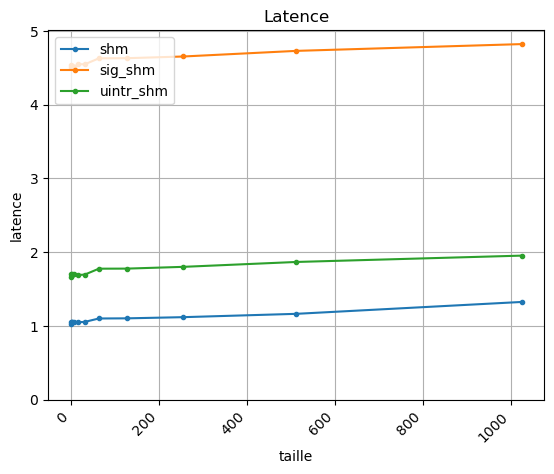
\includegraphics[width=\textwidth]{sendrecvBenchLatency}
  \caption{Latence avec le benchmark \emph{sendrecv}}
  \label{fig:sendrecvBenchLatency}
\end{figure}

Sur la figure \ref{fig:sendrecvBenchThroughput}, nous pouvons observer les courbes de débit du même benchmark.
L'axe des abscisses représente la taille des paquets, et l'axe des ordonnées indique le débit en Mo par seconde.
Grâce à ces courbes de débit, on remarque que le surcoût ajouté par l'utilisation des \uintr{} ou des signaux est constant.

\begin{figure}[H]
  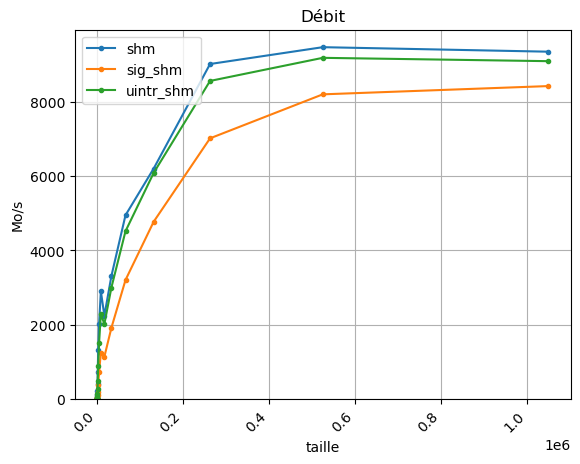
\includegraphics[width=\textwidth]{sendrecvBenchThroughput}
  \caption{Débit avec le benchmark \emph{sendrecv}}
  \label{fig:sendrecvBenchThroughput}
\end{figure}

Ce cas d'attente active est peu représentatif des vraies applications où l'on cherche à recouvrir la latence des communications avec du calcul.
Par conséquent, on accepte de perdre un peu en performances en attente active pour gagner ailleurs.

\subsubsection{Résultats du recouvrement des communications par du calcul}

Dans la plupart des applications HPC, on cherche à recouvrir la latence des communications avec du calcul, c'est ce qu'on appelle l'\emph{overlap} en anglais.
Le comportement souhaité est donc que l'application effectue du calcul en continu, et qu'elle soit interrompue à certains moments pour effectuer les communications.
Un exemple illustratif est présenté dans la figure \ref{fig:appPollingVsUintr} en annexe, où l'on compare une application utilisant le polling avec une autre application utilisant les \uintr{}.

Les figures suivantes mesurent l'\emph{overlap} au niveau de la réception, car actuellement, seul le récepteur est interrompu.
Nous nous concentrerons uniquement sur la partie de gauche de ces figures, qui concerne les tailles inférieures à 16 ko.

Sur la figure \ref{fig:benchOverlapRecvShm}, on peut voir un graphique sous forme de tuile qui représente la taille des messages sur l'axe des abscisses
et le temps de calcul en microsecondes sur l'axe des ordonnées.
Les valeurs dans les coins en haut à gauche et en bas à droite ont tendance à être erronées en raison de la précision de la mesure.
Quand on envoie très peu de données avec un temps de calcul très long, il est compliqué de voir une différence de temps liée à l'envoi.

Les couleurs correspondent à un ratio du temps mesuré de l'exécution moins le plus grand temps entre le temps de calcul et le temps de communication, le tout normalisé à 1.
La couleur noire correspond donc à une valeur de 0, ce qui signifie que l'\emph{overlap} est parfait.
La couleur rouge correspond à 1, donc il n'y a pas d'\emph{overlap},
et la couleur jaune correspond à 2 ou plus, ce qui signifie que l'execution est plus lente que si on n'avait pas essayé de faire d'\emph{overlap}.
Toutes les valeurs entre 0 et 1 qui passent du noir au violet pour arriver au rouge correspondent donc à un \emph{overlap} plus ou moins présent.

Donc, notre figure correspond au benchmark d'\emph{overlap} à la réception avec le driver \emph{shm}.
On peut voir qu'il n'y a pas vraiment d'\emph{overlap} car c'est un driver qui fait seulement de l'attente active.

\begin{figure}[H]
  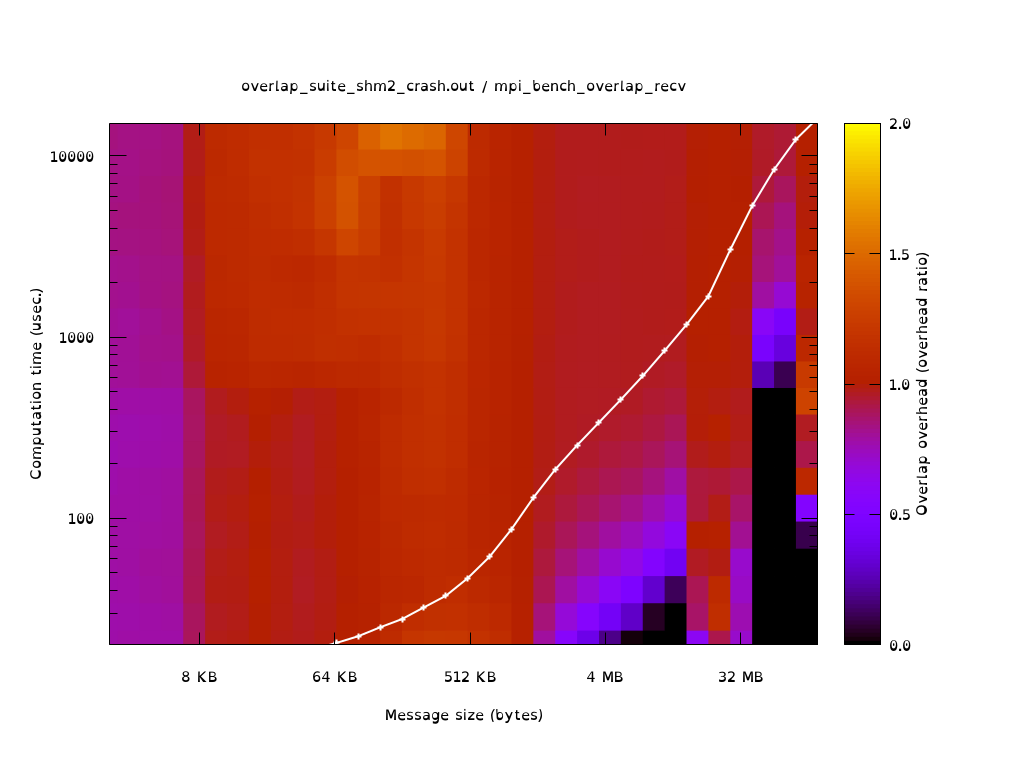
\includegraphics[width=\textwidth]{benchOverlapRecvShm}
  \caption{Benchmark d'\emph{overlap} pour la réception avec le driver \emph{shm}}
  \label{fig:benchOverlapRecvShm}
\end{figure}

Sur la figure \ref{fig:benchOverlapRecvShmUintr}, on peut voir un graphique qui correspond au benchmark d'\emph{overlap} à la réception avec le driver \emph{uintr_shm}.
On remarque que pour les petits paquets, les messages de moins de 16ko, l'\emph{overlap} est presque parfait.
Même pour les plus gros paquets, on constate une légère amélioration car le premier paquet d'entête passe par les petits paquets.
\begin{figure}[H]
  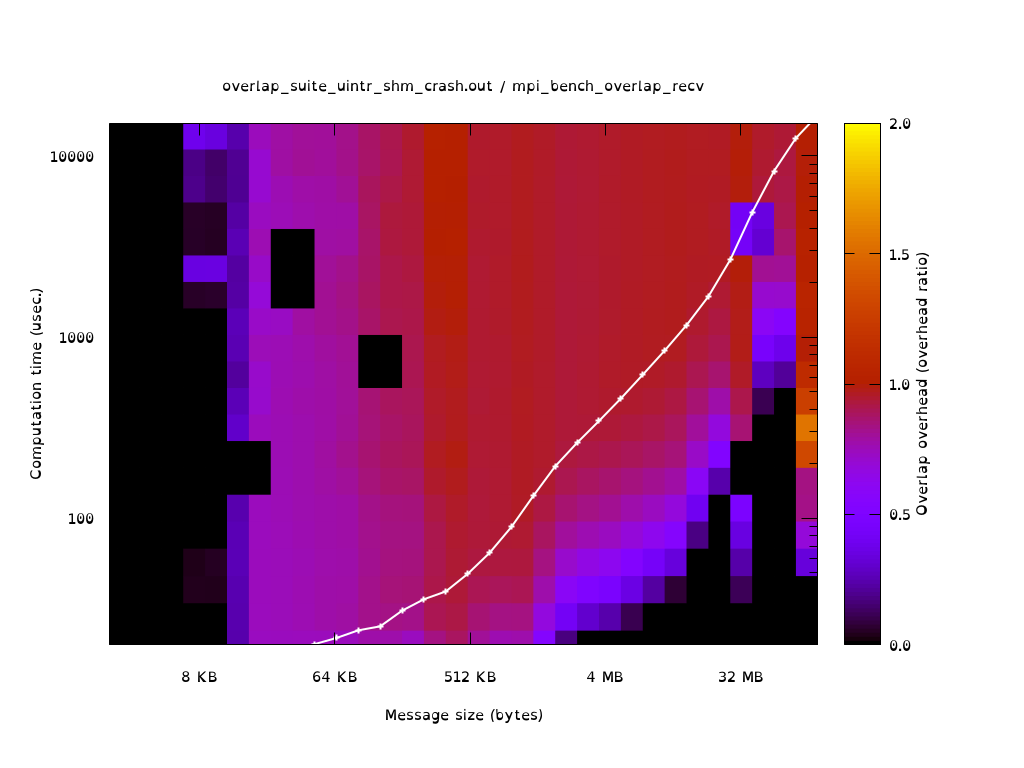
\includegraphics[width=\textwidth]{benchOverlapRecvShmUintr}
  \caption{Benchmark d'overlap pour la réception avec le driver \emph{uintr_shm}}
  \label{fig:benchOverlapRecvShmUintr}
\end{figure}


Ces résultats nous montrent que l'utilisation d'\uintr{} permet effectivement de faire progresser les communications sans recourir au polling,
tout en offrant de bonnes performances.
